\chapter{Производная и дифференциал}
\section{Дифференцируемые функции}
Рассматриваем числовую функцию $f:X\to Y$. Пусть $x_0$ --- предельная точка множества $X$ и $x_0\in X$.\\\\
$\bullet$ \textit{Функцию $f$ будем называть \textbf{дифференцируемой} в точке $x_0$, если существует такое число $A\subset\Rm$, что $\forall h$ такого, что $x_0+h\in X$, выполняется равенство$$f(x_0+h)=f(x_0)+A\cdot h+\alpha(h)\cdot |h|,$$ где $\alpha(h)$ непрерывная в $0$ функция  и $\alpha(0)=0$.}\\\\
Отметим, что $\alpha (h)\to 0$ при $h\to 0$, так как $\alpha$ непрерывна в нуле и $\alpha(0)=0$. На основании этого соображения $\alpha(h)|h|=o(h)$ при $h\to 0$.
Поэтому \textbf{условие дифференцируемости} можно записать в виде
$$f(x_0+h)=f(x_0)+A\cdot h+o(h),\ h\to 0$$
$\bullet$ \textit{Величину $h=(x_0+h)-x_0$ называют \textbf{приращением аргумента} и часто обозначают $\Delta x$, соответственно $f(x_0+h)-f(x_0)=f(x_0+\Delta x)-f(x_0)=\Delta f(x_0)$ называют \textbf{приращением функции}.}\\\\
В соответствии с этими обозначениями условие дифференцируемости функции можно записать так $$\Delta f(x_0)=A \Delta x+o(\Delta x),\ \Delta x\to 0.$$
$\bullet$ \textit{Выражение $A\Delta x=A\cdot h$ называется \textbf{дифференциалом} функции $f$ в точке $x_0$ и обозначается $d f(x_0)$.}\\\\
Таким образом, $$d f(x_0)=A h=A\Delta x.$$
Следовательно, для дифференцируемой функции $$\Delta f=d f +o(\Delta x),\ \Delta x\to 0.$$
Откуда видно, что дифференциал функции представляет собой линейную часть приращения функции.
\begin{theorem}
	Если $f$ дифференцируема в точке $x_0$, то она и непрерывна в точке $x_0$.
\end{theorem}
\begin{Proof}
	$\Delta f\to 0$ при $\Delta x\to 0$.
\end{Proof}\\\\
Мы говорим о дифференцируемости функции и сейчас самое время вспомнить о производной\\\\
$\bullet$ \textit{Предел \[\lim_{\Delta x\to 0}\frac{f(x_0+\Delta x)-f(x_0)}{\Delta x}=\lim_{h\to 0}\frac{f(x_0+h)-f(x_0)}{h}=\lim_{x\to x_0}\frac{f(x)-f(x_0)}{x-x_0},\] если он существует и конечен, называется \textbf{производной} функции $f$ в точке $x_0$ в точке $x_0$ и обозначается одним из следующих символов $$f'(x_0);\quad\frac{d f}{d x}(x_0);\quad\frac{d f(x_0)}{d x};\quad D f(x_0).$$}
\newtheorem*{krdif}{Критерий дифференцируемости функции в точке}
\begin{krdif}
	Для дифференцируемости функции $f$ в точке $x_0$ необходимо и достаточно существование в этой точке конечной производной. При этом $A=f'(x_0)$.
\end{krdif}
\begin{Proof}
	\textbf{Необходимость}. Пусть $f$ дифференцируема в точке $x_0$. Тогда $f(x_0+h)=f(x_0)+A h+ o(h)$,\\ отсюда $$\frac {f(x_0+h)-f(x_0)}{h}=A+\frac{o(h)}{h},$$ \[\lim_{h\to 0}\frac{\Delta f(x_0)}{h}=A \Rightarrow \exists f'(x_0),\] $$f'(x_0)=A.$$
	\textbf{Достаточность}. Пусть $\exists f'(x_0)$. Это значит, что существеут конечный предел \[\lim_{h\to 0}\frac {f(x_0+h)-f(x_0)}{h}=f'(x_0).\]
	Отсюда следует, что $$\frac{f(x_0+h)-f(x_0)}{h}=f'(x_0)+ o(1),\ {h\to 0};$$
	$$f(x_0+h)-f(x_0)=f'(x_0) h+h o(1),\ h\to 0;$$
	$$f(x_0+h)=f(x_0)+f'(x_0) h+ o(h),\ h\to 0.$$ Это  и означает, что $f$ дифференцируема в точке $x_0$ и $A=f'(x_0)$.
\end{Proof}\\\\
С учетом доказанного критерия, дифференциал функции $d f=A h=A \Delta x$ в точке $x_0$ можно записать и в виде $$d f=f'(x_0)\Delta x.$$
Так как для функции $f(x)=x\Rightarrow f'(x_0)=1$, то $$d f(x)=d x=\Delta x.$$
$\bullet$ \textit{Обычно, в связи с этим и для удобства дальнейшего приращение независимого переменного $x$, т.е. $\Delta x$ обозначают $d x$ и называют \textbf{дифференциалом независимого переменного}, то есть $d x$.}\\
Тогда $$d f=f'(x_0) d x.$$
$\bullet$ \textit{Отсюда видно, что $f'(x_0)=\dfrac{d f}{d x}$ --- не только символ производной, но его можно так же трактовать и как \textbf{отношение дифференциалов}.}\\\\
$\dfrac{d f}{d x}$ --- символ, предложенный Лейбницем;\\\\
$f'(x)$ --- символ, предложенный впоследствии Лагранжем.\\\\
В механике, кроме указанных символов используют $\dot\varphi (t)$, если $t$ --- время; в дифференциальной геометрии: $\dot\varphi(s)$, если $s$ --- натуральный параметр.
\section{Односторонние и бесконечные производные.}
Предел
\[\lim_{h\to 0}\frac {f(x_0+h)-f(x_0)}{h}\] может оказаться и бесконечным.\\\\
$\bullet$ \textit{Тогда говорят, что функция $f$ обладает \textbf{бесконечной производной} в точке $x_0$.}\\\\
Если в точке $x_0$ существует бесконечная производная, то функция $f$ не дифференцируема в этой точке.\\\\
Иногда рассматривают и односторонние производные функции $f$ в точке $x_0$.\\
\[f'_+(x_0)=\lim_{h\to +0}\frac {f(x_0+h)-f(x_0)}{h}=\lim_{\Delta x\to +0}\frac {f(x_0+\Delta x)-f(x_0)}{\Delta x}=\lim_{x\to x_0+0}\frac {f(x)-f(x_0)}{x-x_0}\]-- правая производная,
\[f'_-(x_0)=\lim_{h\to -0}\frac {f(x_0+h)-f(x_0)}{h}\] -- левая производная.
\begin{theorem}
	Для дифференцируемости $f$ в т. $x_0$ необходимо и достаточно существование левой и правой производных и их совпадение. При этом $f'_+(x_0)=f'(x_0)=f'_-(x_0).$
\end{theorem}
\begin{Proof}
	Следует из соответствующего свойства пределов.
\end{Proof}\\
\begin{example}
	\[f(x)=|x|,\quad f'_+(0)=\lim_{\Delta x\to +0}\frac {f(0+\Delta x)-f(0)}{\Delta x}=\lim_{\Delta x \to +0}\frac{|\Delta x|}{\Delta x}=1\]
	Аналогично, $f_-'(0)=-1$. Тогда функция не дифференцируема в точке $x=0$.\\\\
	Кроме того, этот пример показывает, что из непрерывности функции не следует дифференцируемость.
\end{example}
\section{Геометрический смысл производной и дифференциала в точке.}
Рассмотрим отношение $\dfrac{\Delta f(x_0)}{\Delta x}=\dfrac{f(x_0+\Delta x)-f(x_0)}{\Delta x}=\tg\varphi_c$, то есть это угловой коэффициент секущей
$$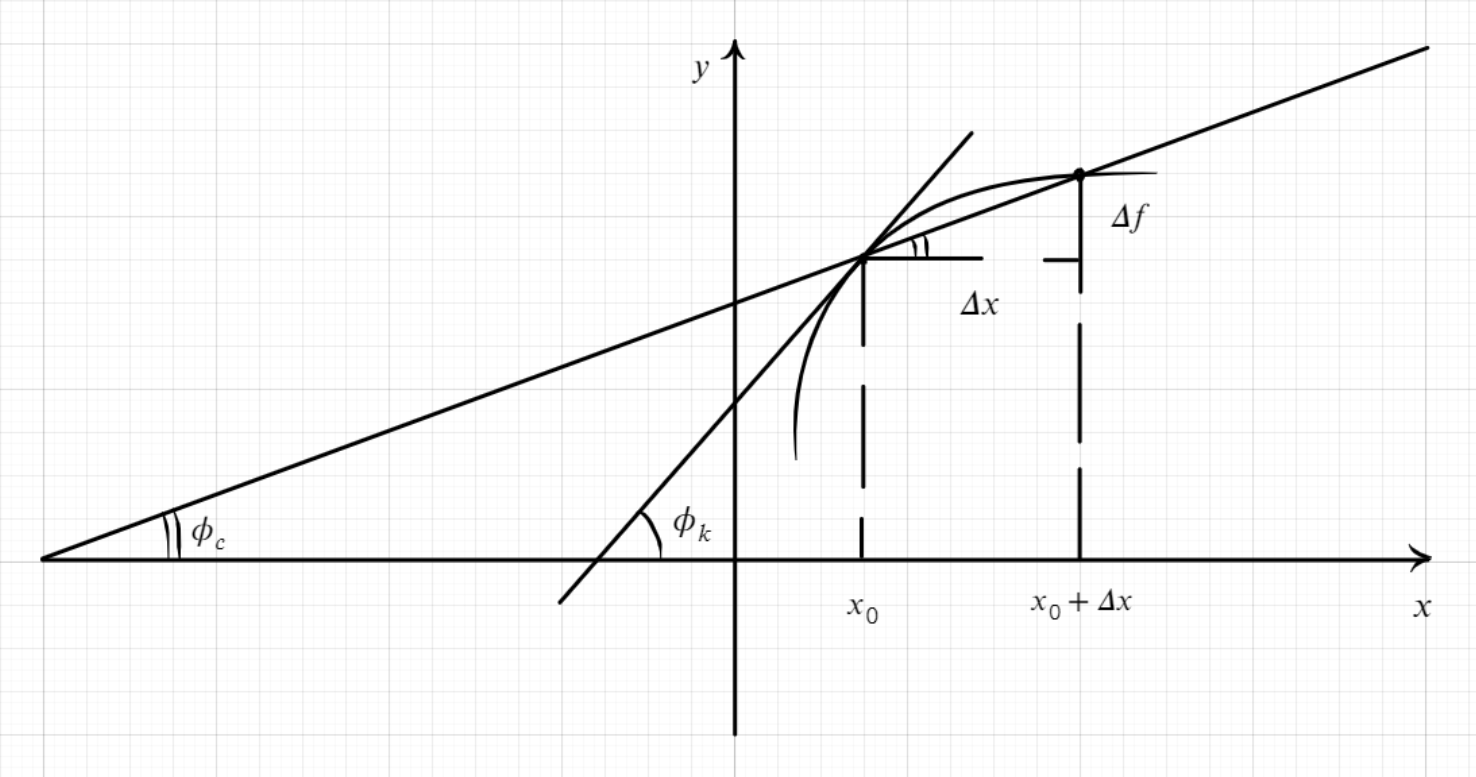
\includegraphics[scale=0.5]{images/img15.png}$$
$\bullet$ \textit{Если существует предельное положение секущей при $\Delta x\to0$, то говорят, что в точке $(x_0;\ f(x_0))$ графика Г$_f$ существует касательная к графику Г$_f$. А само предельное положение секущей называют \textbf{касательной}.}\\\\
Обозначим $\varphi_k$ угол между касательной и положительным направлением оси $Ox$ 
\[\lim_{\Delta x\to 0}\tg\varphi_c=\tg\varphi_k=f'(x_0).\]
Таким образом, если $f$ дифференцируема в точке $x_0$, то есть в этой точке существует конечная производная $f'(x_0)$, то в точке $(x_0;f(x_0))$ графика Г$_f$ функции $f$ существует касательная, причем $\tg\varphi_k=f'(x_0)$.\\\\
Уравнение касательной имеет вид:$$y-f(x_0)=f'(x_0)(x-x_0).$$
Уравнение нормали:$$y-f(x_0)=-\frac{1}{f'(x_0)}(x-x_0).$$
\subsection{Геометрический смысл дифференциала.} $$\Delta f=d f+o(h);\quad d f=f'(x_0)\Delta x=\tg\varphi_k \Delta x.$$
$$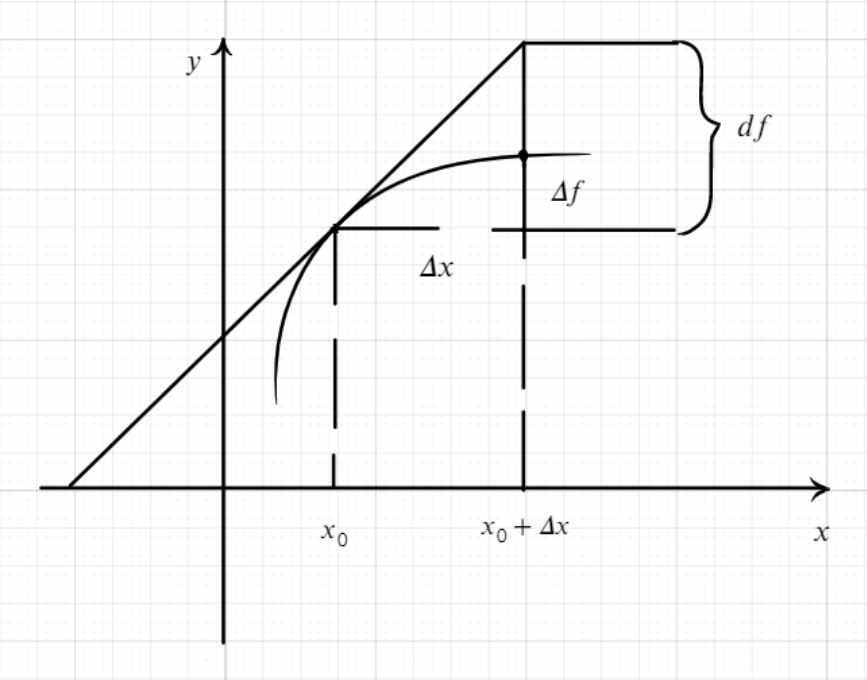
\includegraphics[scale=0.6]{images/img16.png}$$
$\bullet$ \textit{\textbf{Дифференциал} --- это приращение по касательной.}\\\\
Если $h=\Delta x$ --- малое приращение, то дифференциал дает хорошее приближение $\Delta f$, а преимущество дифференциала по сравнению с приращением очевидны:дифференциал от приращения $\Delta x$ зависит линейно, в отличие от $\Delta f$.\\
Итак, при достаточно малых $\Delta x: \Delta f\thickapprox d f$, то есть $$f(x_0+\Delta x)\thickapprox f(x_0)+f'(x_0)\Delta x.$$
Геометрическии это означает, что график функции в некоторой достаточно малой окрестности точки $(x_0;\ f(x_0))$ заменяется графиком касательной. Эта замена с точностью до бесконечно малых более высокого порядка, чем $\Delta x$.\\\\
$\bullet$ \textit{Такая замена называется \textbf{линеаризацией функции}. В этом главная идея дифференциального исчисления: замена функции линейной.}\\\\
Формула $\Delta f\thickapprox d f$ часто используется и для приближенных вычислений значений функции.
\section{Производные арифметических комбинаций.}
\textbf{\textit{Свойства дифференцируемых в точке $x_0$  функции $f$ и $g$:}}
\begin{enumerate}
	\item \textit{$\alpha f+\beta g$, $\alpha, \beta \in \Rm$ также дифференцируема в точке $x_0$, причем $$(\alpha f+\beta g)'(x_0)=\alpha f'(x_0)+\beta g'(x_0);$$}
	\item $$(f g)'(x_0)=f'(x_0)g(x_0)+f(x_0)g'(x_0).$$
	\item $$\Big(\frac{f}{g}\Big)'(x_0)=\frac{f'(x_0)g(x_0)-f(x_0)g'(x_0)}{g^2(x_0) },\quad g(x_0)\not=0.$$
\end{enumerate}
\begin{Proof}
	Доказываются эти свойства по одинаковому принципу. Докажем например, 2.\\\\
	Пусть $\varphi:=f\cdot g$, функция $f$ дифференцируема в точке $x_0 \Rightarrow$ $$f(x_0+h)=f(x_0)+f'(x_0)h+\alpha_1(h)|h|$$
	$g$ дифференцируема в точке $x_0 \Rightarrow$ $$g(x_0+h)=g(x_0)+g'(x_0)h+\alpha_2(h)|h|$$
	Поэтому $$\varphi(x_0+h)=f(x_0+h)g(x_0+h)=$$$$=(f(x_0)+f'(x_0)h+\alpha_1(h)|h|)(g(x_0)+g'(x_0)h+\alpha_2(h)|h|)=$$$$=f(x_0)g(x_0)+(f'(x_0)g(x_0)+g'(x_0)f(x_0))h+(\alpha_2(h)f(x_0)+$$$$+f'(x_0)h\alpha_2(h)+\alpha_1(h)\alpha_2(h)|h|+\alpha_1(h)g(x_0)+g'(x_0)h\alpha_1(h))|h|=$$
	$$=h(x_0)+(f(x_0)g'(x_0)+g(x_0)f'(x_0))h+\gamma(h)|h| $$
	$\Rightarrow h$ дифференцируема и $h'=(f g)'(x_0)=f(x_0)g'(x_0)+g(x_0)f'(x_0)$.
\end{Proof}
\begin{corollary}
	\begin{enumerate}
		\item $$d(\alpha f+\beta g)=\alpha d f+\beta d g;$$
		\item\textit{$$d(f g)=f d g+g d f;$$}
		\item\textit{$$d\Big(\frac{f}{g}\Big)=\frac{g d f-f d g}{g^2}.$$}
	\end{enumerate}
\end{corollary}
Звучит так же, как и для производных. Нужно только слово ``производная'' заменить словом ``дифференциал''.
\section{Дифференцируемость композиции.}
\begin{theorem}
	Пусть: $f:X\to Y$ дифференцируема в точке $x_0\in X, g:Y\to Z$ дифференцируема в точке $t_0=f(x_0)$ тогда функция $h=g\circ f : X\to Z$ дифференцируема, в точке $x_0$, причем$$(g\circ f)'(x_0)=g'(f(x_0))\cdot f'(x_0).$$ 
\end{theorem}
\begin{Proof}
	Доказываем на основании определения дифференцируемости. Рассмотрим $$(g\circ f)(x_0+h)-(g\circ f)(x_0)=g(f(x_0+h))-g(f(x_0))=$$ 
	$$=g(f(x_0)+f'(x_0)h+o(h))-g(f(x_0))=g(t_0+k)-g(t_0)=$$
	$$=g'(t_0)k+g(k)=g'(t_0)(f'(x_0)h+o(h))+o(f'(x_0)h+o(h))=$$
	$$=f'(x_0)g'(t_0)h+o(h),\ h\to 0 \Rightarrow$$
	$g\circ f$ дифферецируема в точке $x_0$ и $$(g\circ f)'(x_0)=f'(x_0)\cdot g(f(x_0)).$$
\end{Proof}
\begin{corollary}
	Это правило вычисления композиции называют правилом цепочки. Оно имеет место для любого конечного числа функций.
\end{corollary}
\begin{example}
	$(f\circ g \circ h)'(x_0)=f'((g\circ h)(x_0))\cdot g'(h(x_0))\cdot h'(x_0)$
\end{example}
\begin{corollary}
	В условиях теоремы $$d(g\circ f)(x_0)=g'(f(x_0))\cdot f'(x_0)\dx.$$
\end{corollary}
\section{Инвариантность формы первого дифференциала.}
Пусть функция $g: Y\to Z$ дифференцируема в точке $y_0\in Y$ тогда, как уже отмечалось, $$d g=g'(y_0)d y,$$ где $d y=\Delta y$ --- приращение аргумента функции $y$.\\\\
Если $y=f(x)$, то есть $y$ --- зависимая переменная, то есть функция независимого переменного $x$, а функция $f: X\to Y$ дифференцируема в точке $x_0, y_0=f(x_0)$, то $$d g=d((g\circ f))=(g\circ f)'(x_0)d x=g'(y_0)\cdot f'(x_0)d x=g'(y_0)d y,$$ где $d y$ --- дифференциал функции $f$.\\\\ Таким образом:\\\\
\textit{Форма дифференциала первого порядка (первого дифференциала) $d g=g'(y_0)d y$ не зависит (инвариантна) относительно того, является ли $y$ независимой переменной или функцией некоторого аргумента}. \\\\
Следует только иметь ввиду, что если $y$ --- независимая переменная, то $dy = \Delta{y}$, а если $y$ --- функция, то $dy = df$. Содержание формулы $dg = g^\prime{(y_0)}dy$ различно в этих двух случаях, но вид формулы, её форма одинаковы. В связи с этим и говорят, что дифференциал первого порядка обладает инвариантностью формы.
\section{Дифференцируемость обратной функции.}
\newtheorem*{t1_1}{Теорема о производной обратной функции}
\begin{t1_1}
	Пусть функция $f : [a; b] \rightarrow E$ строго монотонна, непрерывна на $[a; b]$ и дифференциируема во внутренней точке $x_0 \in ]a ; b[$ и $f^\prime{(x_0)} \not= 0$.
	Тогда обратная функция $f^{-1} : E \rightarrow [a; b]$ дифференцируема в точке $y_0 = f(x_0)$, причем $(f^{-1})^\prime(y_0) = \dfrac{1}{f^{\prime}(x_0)}.$
\end{t1_1}
\begin{Proof}
	По критерию непрерывности монотонной функции $E(f) = [A; B]$. По теореме об обратной функции, обратная функция $f^{-1} : [A; B] \rightarrow [a; b]$ является строго монотонной и непрерывной.
	\\\\
	Найдем предел $\lim\limits_{\Delta{y} \to 0} \dfrac{f^{-1}(y) - f^{-1}(y_0)}{y - y_0} = [$ но $f^{-1}(y) = x, f^{-1}(y_0) = x_0, y = f(x), y_0 = f(x_0) ] = \lim\limits_{\Delta{y} \to 0} \dfrac{x - x_0}{f(x) - f(x_0)} = [$ т.к. обратная функция непрерывна, то $\Delta{y} \rightarrow 0 \Rightarrow \Delta{x} \rightarrow 0 ] = \lim\limits_{\Delta{x} \rightarrow 0} \dfrac{x - x_0}{f(x) - f(x_0)} = \lim\limits_{\Delta{x} \rightarrow 0} \dfrac{1}{\frac{f(x) - f(x_0)}{x - x_0}} = \dfrac{1}{f^\prime(x_0)}.$\\\\
	Это и означает, что $f^{-1}$ дифференциируема и $$(f^{-1})(y_0) = \frac{1}{f^\prime(x_0)}.$$
\end{Proof}
\textbf{Замечание.} Иногда удобнее пользоваться формулой, записанной в таком виде
$$(f^{-1})(y_0) = \frac{1}{f^\prime(f^{-1}(y_0))}.$$
\textbf{Замечание.} Так как $(f^{-1} \circ  f)(x) = x$, то применение теоремы о дифференциировании композиции приводит к нужному результату $$f^{{-1}^\prime}(f(x)) \cdot f^\prime(x) = 1 \Rightarrow (f^{-1})^\prime(y_0) = \frac{1}{f^\prime(x_0)}.$$
\subsection{Геометрический смысл теоремы.}
$$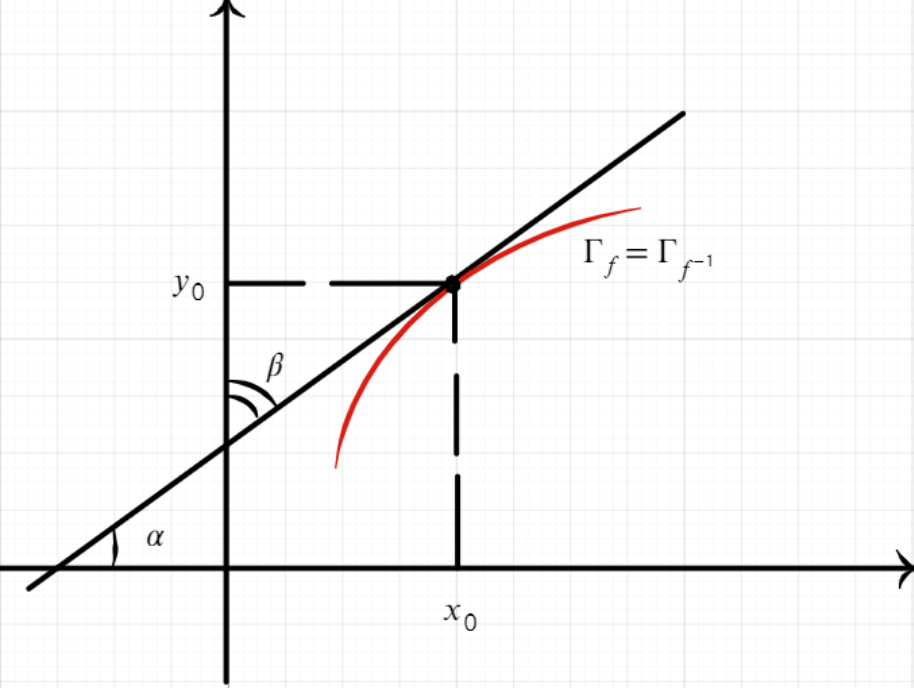
\includegraphics[scale=0.5]{images/img17.png}$$
$\tg \alpha  = f'(x_0)$, $\tg \beta = (f^{-1})'(y_0)$, но $\alpha + \beta = \frac{\pi}{2}\Ra \beta = \frac{\pi}{2}-\alpha\Ra (f^{-1})'(y_0) = \tg \beta= \tg (\frac\pi2 - \alpha) = \ctg \alpha = 1/\tg \alpha = 1/f^{-1}(x_0)$.\\\\
 Можно и чуть иначе.
 $$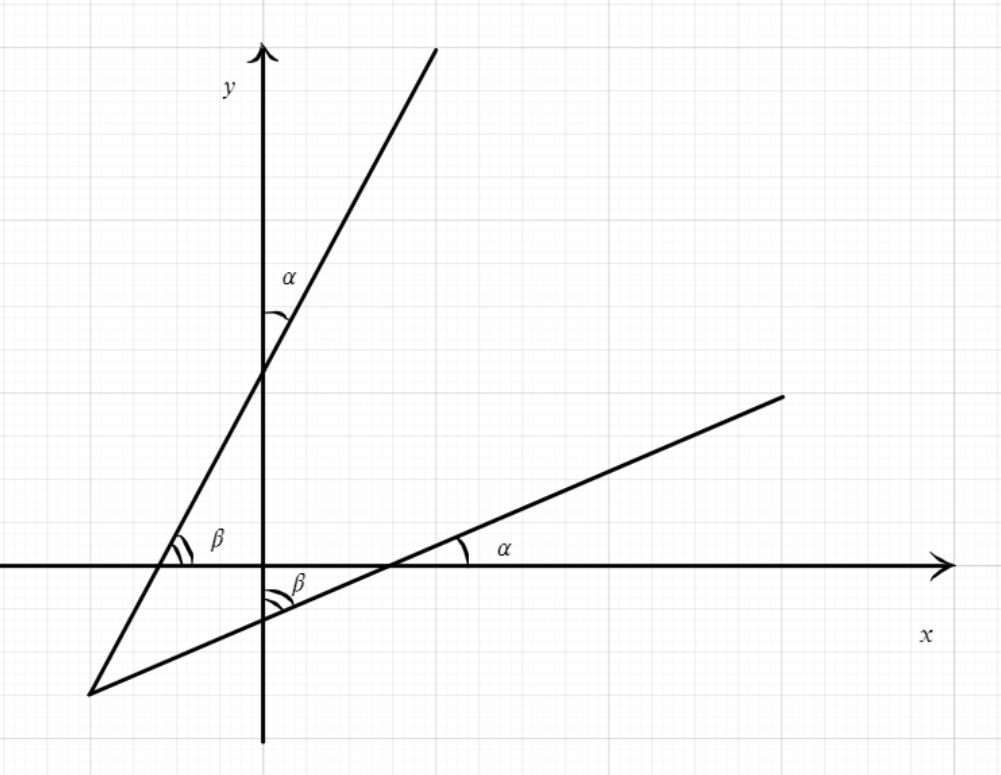
\includegraphics[scale=0.5]{images/img18.png}$$
 $\beta = \frac{\pi}{2}-\alpha\Ra (f^{-1})'(y_0) = \tg \beta= \tg (\frac\pi2 - \alpha) = \ctg \alpha = 1/\tg \alpha = 1/f^{-1}(x_0)$.\\
\begin{example}
	\begin{enumerate}
		\item $f = \sin x$, $f^{-1} = \arcsin x -1 < x < 1$.\\\\
		$(\arcsin)^\prime(x) = \dfrac{1}{\sin^\prime(\arcsin(x))} = \dfrac{1}{\cos(\arcsin(x))} = \dfrac{1}{\sqrt{1 - \sin^2(\arcsin(x))}} = \dfrac{1}{\sqrt{1 - x^2}}.$
		\item $f = \tg x, f^{-1} = \arctg x$\\\\
		$\arctg^\prime(x) = \dfrac{1}{\tg^\prime(\arctg(x))} = \cos^2(\arctg(x)) = \dfrac{1}{1 + \tg^2(\arctg(x))} = \dfrac{1}{1 + x^2}.$
		\item $f = \sh x, f^{-1} = \operatorname{arcsh} x;$ т. к. $(\sh(x))^\prime = \frac{e^x + e^{-x}}{2} = \ch(x)$, то\\\\
		$\operatorname{arcsh}^\prime(x) = \dfrac{1}{\sh^\prime( \operatorname{arcsh}(x))} = \dfrac{1}{\ch( \operatorname{arcsh}(x))} = \dfrac{1}{\sqrt{1 + \sh^2(\operatorname{arcch}(x)}} = \dfrac{1}{\sqrt{1 + x^2}}.$
	\end{enumerate}
	Кстати, отсюда следует $(\ln(x + \sqrt{x^2 + 1}))^\prime = \dfrac{1}{\sqrt{1 + x^2}}$\\
	Аналогично: $ \operatorname{arcch}_-(x) = \ln|x - \sqrt{x^2 - 1}|$;  $(\operatorname{arcch}_-(x))^\prime = -\dfrac{1}{\sqrt{x^2 - 1}}$.\\ 
	$\operatorname{arcch}_+(x) = \ln|x + \sqrt{x^2 + 1}|$; $(\operatorname{arcch}_+(x))^\prime = \dfrac{1}{\sqrt{x^2 + 1}}$.
\end{example}
\section{Класс дифференциируемых функций.}
Пусть задана функция $f : X \rightarrow Y$. Мы можем поставить вопрос о дифференциируемости $f$ в любой внутренней точке множества $X$.\\\\
$\bullet$ \textit{Если у множества все точки внутренние, то оно называется \textbf{открытым}.}\\\\
Пусть $X$ --- открытое множество и $f$ дифференциируема во всех точках множества $X$. \\\\
$\bullet$\textit{ Тогда говорят, что $f$ \textbf{дифференциируема на множестве} $X$. Множество всех дифференциируемых на $X$ функций будем обозначать $D(X)$. Запись $f \in D(X)$ означает, что $f$ диффренциируема в каждой точке множества $X$.}\\\\
Заметим, что $f \in D(X) \Rightarrow f \in \mathcal{C}(X)$.\\\\
Если $f$ определена на  $[a; b]$, то будем говорить, что $f \in D([a; b])$ , если $f$ дифференциируема во всякой внутренней точке, т. е. на $]a; b[$ а в точках $a$ и $b$ существуют соответственно правая и левая производные, т. е. $f_+^\prime(a)$ и $f_-^\prime(b)$.\\\\
Пусть $f \in D(X)$. Тогда на множестве $X$ автоматически строится новая функция $f^\prime$, которая каждой точке $x \in X$ ставит в соответствие производную $f^\prime(x) : f^\prime : x \rightarrow f^\prime(x)$.\\\\
Эту функцию называют производной от функции $f$. Если $f^\prime$ непрерывна на $X$, т. е. $f^\prime \in \mathcal{C}(X)$, то говорят, что $f$ непрерывно дифференциируема на $X$ и пишут $f \in \mathcal{C}^1(X)$, т. е. класс непрерывно дифференциируемых функций обозначают $\mathcal{C}^1(X)$. Очевидно, что $\mathcal{C}^1(X) \subset D(X)$, т. е. из $f \in \mathcal{C}^1(X) \Rightarrow f \in D(X)$.\\\\
Обратное, вообще говоря, не верно.
\section{Векторные функции.}
$\bullet$\textit{ Фунцкию $\vec{r} = \vec{r}(t)$\textbf{ называют дифференциируемой в точке} $t_0$, если $\exists \vec{A} \in \Rm^3$, что для $\forall h, t_{0+}h \in D(\vec{r}) \Rightarrow \vec{r}(t_{0+}h) = \vec{r}(t_0) + \vec{A}h + \vec{0}(h), h \rightarrow 0$}.
\textit{Производная}: $$\vec{r}^\prime(t_0) = \lim_{\Delta t \rightarrow 0} \frac{\vec{r}(t_0 + \Delta t) - \vec{r}(t_0)}{\Delta t}$$\\\\
\textit{Для дифференциируемости $\vec{r}(t)$ в точке $t_0$ необходимо и достаточно дифференциируемость в этой точке функций $x(t), y(t), z(t)$. При этом:}\\
$$\vec{r}(t_0) = (x^\prime(t_0), y^\prime(t_0), z^\prime(t_0).$$
Совершенно аналогично определяются и векторные функции $f : X \longrightarrow \Rm^n$\\
вектор $\leftrightarrow$ точка пространства $\Rm^n \leftrightarrow$ набор из $n$ чисел.\\
$$f(x) = (f_1(x), f_2(x), \dots, f_n(x)).$$
$f_i(x)$ --- координатные функции векторной функции векторной функции $f$.\\
Обычным образом вводится понятие предела, только вместо модулей расстояние $\rho$
$$\rho(x_1, x_2) = \sqrt{\sum_{k = 1}^n(x_1^{(k)} - x_2^{(k)})}.$$
\subsection{Комплекснозначные функции.}
Дифференцирование вводится обычным образом.

\section{Производные и дифференциалы высших порядков.}
Если функция $f : x \rightarrow \Rm$ дифференцируема в любой точке $x \, \in X$, то на множестве $X$ можно построить новую функцию $f' : x \longrightarrow \Rm$, значения которой в точке $x \in X$ равно значению производной функции $f$, то есть $f'(x)$.\\\\
$\bullet$ \textit{Если $f^\prime$ дифференцируема в некоторой точке $a \in X$, то производную от $f^\prime$ в точке $a$ называют \textbf{второй производной} от $f$ в точке $a$ и обозначают символом $f"(a), f^{(2)}(a), \dfrac{d^2f}{d x^2}(a) \, , \, D^2f(a)$}.\\\\
Итак, по определению $f"(a)=(f')'(a)$.\\\\
Чтобы построить $f"(a)$ достаточно, чтобы $f$ была дифференцируема не только в точке $a$, но и в некоторой окрестности этой точки.
Легко видеть. что если $f$ дважды дифференцируема в точке $a$, то $f^\prime$ непрерывна в т. $a$.\
Если $f$ дважды дифференциируема в каждой точке $x \in X$, то можно построить функцию
$$f" : X \rightarrow \Rm, \, \, f" : x \mapsto f"(x).$$
Далее такой же подход позволяет построить $f'''$(если это позволяет функция $f$) и так далее.
Производная $n-$го порядка определяется индуктивно
$$f^{(n)}(x)=(f^{(n-1)})'(x) \quad \Big( \frac{d^n f}{d x^n}, \, \, D^n  f\Big).$$
Класс $n$ раз дифференцируемых на $X$ функций обозначают $D^n (X)$
$$f \in D^n(X) \, \Longrightarrow \, f \in \mathcal{C}^{n-1}(X).$$
$\mathcal{C}^n(X)$ --- класс $n$ раз непрерывно дифференцируемых функций.
$$\mathcal{C}^n(X) \subset D^n(X), \quad \mathcal{C}^0(X)=\mathcal{C}(X).\quad f^{(0)}=f$$
Аналогичным образом определяются и дифференциалы высших порядков. Мы умеем вычислять дифференциал первого порядка
$df=f'(x)dx.$ Предположим. что $f \in D^n(X)$ и положим $d^2f ::=d(d f)$.
$df$ --- функция двух переменных
$$d^n f ::=d(d^{n-1} f).$$
Изучим $d^2f$ в предположении, что $x$ --- независимая переменная. $df=f'(x)dx,$ причем $dx= \Delta x$ --- не зависит от $x$, если $x$ --- независимый аргумент, то есть по отношению к $x$ операции дифференцирования $dx$ считаем постоянной.\\\\
$d^2f=d(df)=d(f'(x)dx)=f''(x)dx \cdot dx =f''(x) d x^2$,\\
$dx \cdot dx=(dx)^2= :: d x^2$.\\\\
Если $x$ --- независимая переменная, то $d^k x=0, \, \, k>1$
Аналогично получаем
$$d^n f=f^{(n)}(x) d x^n ; \quad f^{(n)}(x)=\frac{d^n f}{d x^n}.$$
Интересно посмотреть, что будет в случае, если $x$ --- не является независимой, то есть $x$ есть функция другого аргумента.\\\\
В силу инвариантности формы первого дифференциала $df=f'(x)dx,$ однако здесь $dx$ уже не приращение аргумента, не постоянная, а дифференциал функции, то есть функция некоторой переменной\\\\
Сосчитаем $d^2f$:
$$d^2f=d(df)=d(f^\prime(x)dx)=d(f^\prime(x))dx+f^\prime(x)d(dx)=f^{\prime\prime}(x) d x^2+f^\prime(x) d^2 x.$$
Здесь уже $d^2x$ не обязано быть тождественным нулем. Отсюда вывод:\\\\
\textit{Форма дифференциала второго порядка функции $f$ меняется в зависимости от того: $x$ --- независимая переменная или $x$ --- промежуточный аргумент}.\\\\
Те же выводы справедливы и относительно дифференциала $n-$го порядка.\\\\
Однако форма $n-$го дифференциала не меняется, если промежуточный аргумент $x$ зависит от окончательного аргумента $t$, линейно: $x=at+b$.
\section{Производныe и дифференциалы высших порядков элементарных функций.}
\begin{enumerate}
	\item $f(x)=x^{\mu}$.\\\\
	$f^\prime(x)=\mu x^{\mu - 1}, \dots , f^{(n)}(x)=\mu(\mu - 1)\dots(\mu - n + 1)x^{\mu - n}$.\\\\
	Если $\mu = m \in \N$, то для $n > m (x^m)^n = 0, (x^m)^m = m$.
	\item $f(x) = \ln x$.\\\\
	$f^\prime(x) = \dfrac{1}{x} = x^{-1}$.\\\\
	$f^{(n)}(x) = (x^{-1})^{(n - 1)} = (-1)(-2)\dots(-n+1)x^{-n + 1 \not = 1}$.
	$$(\ln x)^{(n)} = (-1)^{n - 1}(n - 1)!\cdot x^{-n}.$$
	\item $f(x) = a^x$. $(a^x)^{(n)} = a^xln^na$, $(e^x)^{(n)} = e^x$.
	\item $f(x) = \sin x$.\\\\
	$f^\prime(x) = \cos x; f^{\prime\prime}(x) = -\sin x, f'''= -\cos x, f''''(x) = \sin x$.\\\\
	\begin{Proof}
		Предположение $f^{(n)}(x) = \sin(x + \frac{\pi n}{2})$.\\\\
		Индукция: $n = 1$ $(\sin x)^{(n + 1)} = ((\sin x)^{(n)})' = \sin'(x + \frac{\pi n}{2}) = \cos(x + \frac{\pi n}{2}) = \sin(x + \frac{\pi n}{2} + \frac{\pi}{2}) = \sin(x + \frac{\pi (n + 1)}{2}) \Rightarrow$ гипотеза верна. 
		\end{Proof}
	\item $f(x) = \cos x$. $(\cos x)^{(n)} = \cos(x + \frac{\pi n}{2}$.
	\item $f(x) = \sh x$. $(\sh x)^{(n)} = \begin{cases} \sh x, n = 2k\\ \ch x, n = 2k - 1\end{cases}$.
	\item $f(x) = \ch x$. $(\ch x)^{(n)} = \begin{cases} \ch x, n = 2k\\ \sh x, n = 2k - 1 \end{cases}$.
\end{enumerate}
\section{Производные и дифференциалы n-го порядка арифметических комбинаций.}
Далее предполагаем, что $u, v \in D^n(x)$. Тогда
\begin{enumerate}
	\item $(\alpha u + \beta v)^{(n)^\prime} = \alpha u^{(n)} + \beta v^{(n)};$\\
	$d^n(\alpha u + \beta v) = \alpha d^nu + \beta d^nv.$
	\begin{Proof}
		Доказывается по индукции.
	\end{Proof}
	\item \textbf{Правило Лейбница.}
	$$(uv)^{(n)} = \sum^n_{k = 0} C^k_n u^{(n-k)} v^{(k)}.$$
	\textit{Используется для вычисления $n$-ой производной произведения.}
	\begin{Proof}
		Доказываем по индукции.\\
		При $n=1$:  
		$$(uv)' = C^0_1 u' v^{(0)} + C^1_1 u^{(0)} v' \Leftrightarrow (uv)' = u'v + uv'$$ --- известная нам формула. \\\\
		Предположим, что формула справедлива при $n = m$, то есть 
		$$(uv)^{(m)} = \sum^m_{k = 0} C^k_m u^{(m-k)} v^{(k)}.$$
		Тогда $$(uv)^{(m+1)} =((uv)^{(m)})' = (\sum^m_{k = 0} C^k_m  u^{(m-k)} v^{(k)})' = $$ 
		$$= \sum^m_{k = 0} C^k_m (u^{(m-k)} v^{(k)})' = \sum^m_{k = 0} C^k_m (u^{(m-k+1)} v^{(k)} + u^{(m-k)} v^{(k+1)})' = $$ 
		$$= \sum^m_{k = 0} C^k_m u^{(m-k+1)} v^{(k)} + \sum^m_{k = 0} C^k_mu^{(m-k)} v^{(k+1)} =$$ 
		$$= C^0_m u^{(m+1)} v^{(0)} + \sum^m_{k = 1} C^k_mu^{(m-k+1)} v^{(k)} +
		C^m_m u^{(0)} v^{(m+1)} + \sum^{m-1}_{k = 1} C^k_mu^{(m-k)} v^{(k+1)} =$$
		\begin{center}
			= [замена во второй сумме: $k + 1 =: k'$] =
		\end{center}
		$$= u^{(m+1)} v + \sum^m_{k = 1} C^k_mu^{(m-k+1)} v^{(k)} +
		\sum^{m}_{k = 1} C^{k - 1}_m u^{(m-k+1)} v^{(k)} + u v^{(m+1)} =$$ 
		$$= u^{(m+1)} v + \sum^m_{k = 1}(C^{k}_m + C^{k - 1}_m) u^{(m-k+1)}v^{(k)} + u v^{(m+1)} = $$
		$$ = u^{(m+1)} v + \sum^m_{k = 1}C^{k}_{m + 1} u^{(m+1-k)} v^{(k)} + u v^{(m+1)} = $$
		$$ \sum^{m + 1}_{k = 0}C^{k}_{m + 1} u^{(m+1-k)} v^{(k)}.$$
	\end{Proof}
\end{enumerate}
Из этой формулы следует \textbf{формула для дифференциалов }
$$ d^n(uv) = \sum^{n}_{k = 0}C^{k}_{n} d^{(n - k)} u d^{(k)}v.$$
\section{Производная неявной функции.}
Пусть задано соотношение $\F(x,y) = 0$, то есть рассматриваем пары действительных чисел, удовлетворяющих этому сотношению.
\\\\   Допустим, что существует такое множество $X \subset \Rm$, что для каждого $x \in X$ существует по крайней мере одно $y$ такое, что $\F(x,y) = 0$.
\\\\   Выбирая для каждого $x \in X$ только одно фиксированное $y$ из числа возможных, мы приходим к функции $f: X \rightarrow Y  (y \in Y).$
\\\\   Если эту функцию представить в $\F(x,y) = 0$, то из способа построения $f$ вытекает, что $\F(x,f(x)) = 0, \forall x \in X$, то есть получаем тождество.
\\\\  $\bullet$ \textit{Построенную таким образом функцию $f$ называют \textbf{неявной функцей}, или, более точно, говорят, что $f$ задана неявно соотношением $\F(x,y) = 0$.}
\\\\  $\bullet$ \textit{Уравнение $\F(x,y) = 0$ называют также \textbf{функциональным уравнением}}.
\\\\   Функциональные уравнение $\F(x,y) = 0$ может не задавать ни одной функции, одну, две, ..., бесчисленное множество.
\\\\   Такое задание охватывает большее число функций, чем явное задание. Например, $y = f(x)$ явное задание всегда можно записать как $y - f(x) = 0$ - неявное задание.
\\\\   Термин $"$неявная функция$"$ отражает не характер функции, а только способ её задания. 
\\\\   Дифференцируя тождество $\F(x,f(x)) = 0$, получаем уравнение относительно $f'$, причем оно всегда линейное относительно $f'$. Решая это уравнение, находим производную $f'$, которая выражается через $x$ и $f$. Последующие дифференцирования дают возможность находить произведение более высоких порядков.
\\  \begin{example}
	$$\frac{x^2}{a^2} + \frac{y^2}{b^2} = 1.$$ 
	Считаем, что это ФУ, определяет $y = y(x)$. 
	$$\frac{2x}{a^2} + \frac{2yy'}{b^2} = 0 \Rightarrow y' = -\frac{b^2x}{a^2y}.$$
	Чтобы найти вторую производную, дифференциируем повторно 
	$$\frac{2}{a^2} + \frac{2(y')^2}{b^2} + \frac{2yy''}{b^2} = 0 \Rightarrow y'' = -\frac{b^2}{2y}\Big(\frac{2}{a^2} + \frac{2(y')^2}{b^2}\Big) = -\frac{b^2}{y}\Big(\frac{1}{a^2} + \frac{b^4}{b^2a^4}\frac{x^2}{y^2}\Big) = -\frac{b^2}{a^2y} - \frac{b^4}{a^4}\frac{x^2}{y^3}$$
	Аналогично находятся производные более высоких порядков. 
	\\\\Похожим образом обстоит дело и с дифференциалами $$\frac{2xdx}{a^2} + \frac{2ydy}{b^2} = 0 \Rightarrow dy = ... $$ и так далее. Это эллипс 
	$$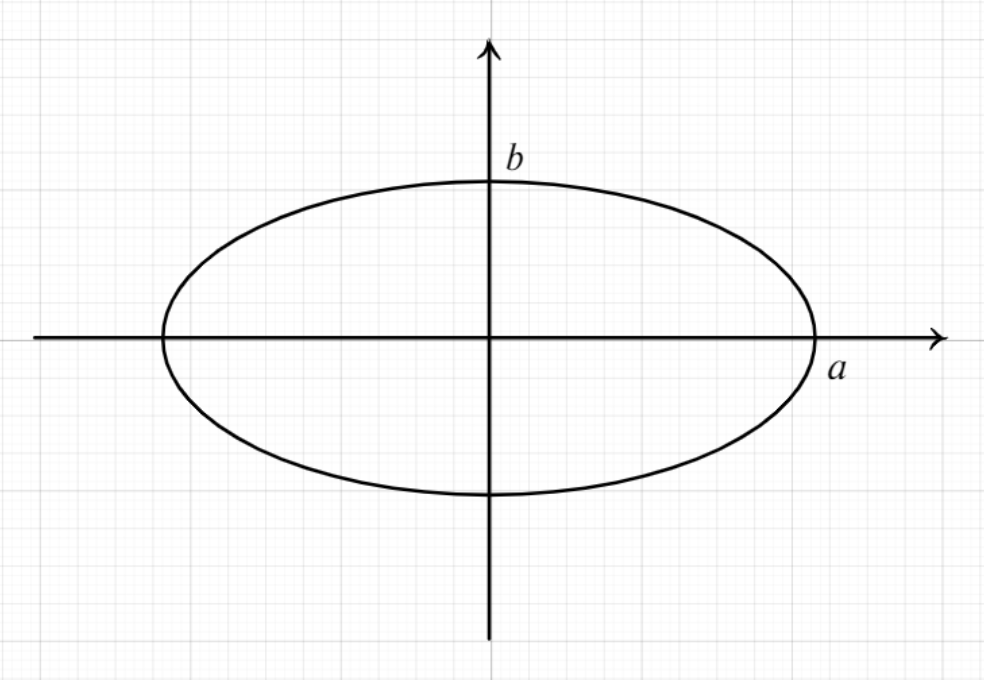
\includegraphics[scale=0.5]{images/img19.png}$$
\end{example}
\section{Производная функции, заданной параметрически.}
Рассмотрим функции
$\begin{cases}
	x = \upvarphi(t), \\
	y = \Psi(t),
\end{cases}   t \in [\alpha,\beta].$   \\\\
Предположим, что функция $\upvarphi$ обратима, то есть уравнение можно разрешить относительно $t : t = \varphi ^{-1}(x)$. Подставим её во второе уравнение, получим $ y = \varphi (\varphi ^{-1}(x)) = :: f(x)$.\\\\
\\То есть, оказывается, что в этом случае определяется функция $y = y(x)$.\\\\
$\bullet$\textit{ Эту функцию называют \textbf{функцией, заданной параметрически} с помощью соотношений }
$\begin{cases} 
	x = \varphi (t), \\
	y = \Psi(t).
\end{cases}$ \\\\
Если дополнительно потребовать, чтобы $x(t), y(t) \in D(|\alpha,\beta|)$, причём $\varphi '(t)  0, \forall t \in |\alpha,\beta|$, то тогда  
$$y' = \Psi(\varphi ^{-1}(x))(\varphi ^{-1})'(x)) = \Psi'(t)\frac{1}{\varphi'(x)} = \frac{\Psi'(t)}{\varphi '(x)}.$$
\\При нахождения производной функции заданной параметрически можно пользоваться инвариантностью формы первого дифференциала \\
$$y'(x) = \frac{dy}{dx} = \frac{\Psi'(t)dt}{\varphi 'dt} = \frac{\Psi'(t)}{\varphi'(t)}.$$
(Доказывать так нельзя, так как $dt$ в числителе и знаменателе, вообще говоря, разные.) \\\\
Иногда записывают так 
$$\begin{cases}
	x = x(t), \\
	y = y(t),
\end{cases}   y'_x  = \frac{y'_t}{x'_t} = \frac{\dot y}{\dot x}.$$
Производные более высоких порядков считаем также по этому правилу
$$y''_{x^2} = (y'_x)'_x = \frac{(y'_x)'_t}{x'_t} = \frac{y''_{t^2}x'_t - x''_{t^2}y'_t}{(x'_t)^3}.$$
Дело в том, что производная определяется двумя равенствами  
$$\begin{cases}
	y = y'_x, \\
	x = x(t).
\end{cases}$$
\\\begin{example}
	Циклоида 
	$$\begin{cases}
		x = a(t - \sin t) \\
		y = a(1 - \cos t)
	\end{cases}$$
	$$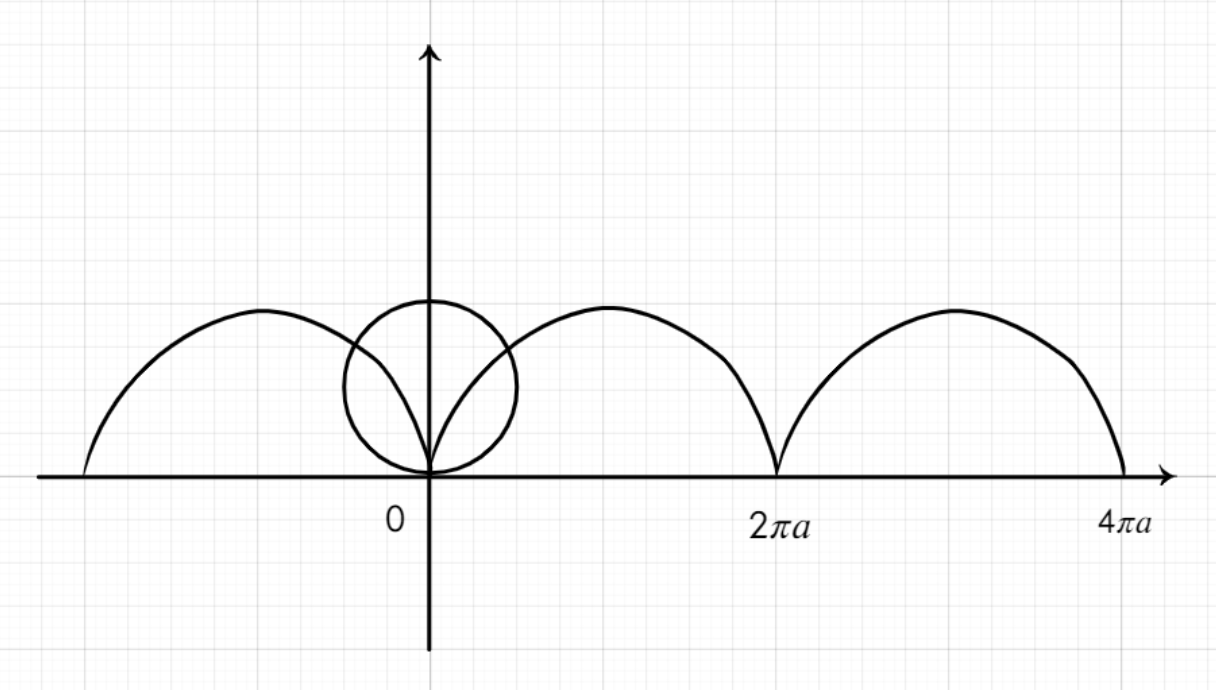
\includegraphics[scale=0.5]{images/img20.png}$$
	$$y'_x = \frac{a\sin t}{a(1 - \cos t)} = \frac{2\sin\frac{t}{2}\cos\frac{t}{2}}{a(1 - \cos t)} = \frac{2\sin\frac{t}{2}\cos\frac{t}{2}}{2\sin^2\frac{t}{2}} = \ctg\frac{t}{2}.$$
\end{example} 
\section{Теорема Вейерштрасса.}
Рассматриваем числовую функцию $f: X \rightarrow \Rm$. Нас будет интересовать экстремальные значения $f$ на множестве $X$, то есть $\min f(x)$ и $\max f(x)$. Эти значения, то есть экстремальные элементы множества задания могут как существовать, так и не существовать. Например, $f(x) = x^2, X = [-1; 2)$ или $f(x) = 0$, $\max f(x) - \nexists$. Однако есть ситуации, когда экстремальные элементы заведомо существуют. Как раз об одной такой ситуации и идёт речь тереме Вейерштрасса.  
\newtheorem*{theor}{Теорема Вейерштрасса}\begin{theor}
	Всякая непрерывная на отрезке $[a; b]$ функция достигает на нем экстремальных значений. 
	Подробнее: если $f \in C([a; b])$, то
	$$\exists \overline{x} \in [a; b], f(\overline{x}) = \max f([a; b]) = \sup f([a; b]);$$
	$$\exists \underline{x} \in [a; b], f(\underline{x}) = \min f([a; b]) = \inf f([a; b]).$$
\end{theor}
\begin{Proof}
	Докажем, например, что достигается максимальное значение. \\\\
	Обозначим $M::= \sup{f(x)} = \sup f([a;b]), x \in [a;b] $ \\\\
	Множество $f([a;b])$ не пусто, так как это множество значений функции, а потому $f([a;b])$ обладает верхней границей, то есть $M$ существует, конечное или бесконечное (нам нужно показать, что $M$ конечно что существует $\overline{x} \in [a;b]$, что $f(\overline{x}) = M$). \\\\
	Построим последовательность $(\alpha_n)$ такую, что $\lim\limits_{n\rightarrow \infty}\alpha_n = M, \alpha_n < M$ для $\forall n \in \N$. \\\\
	В качестве $(\alpha_n)$ можно взять $(\alpha_n) = M - \dfrac{1}{n}$, при $M$ конечном и $(\alpha_n) = n$ при $M\rightarrow +\infty$. 
	Так как $M = \sup f([a;b])$, то $\alpha_n$ при $\forall n$ не является мажорантой. Поэтому для $\forall n$ $\exists x_n \in [a;b]$ такое, что $f(x_n) > \alpha_n$. \\\\
	Рассмотрим последовательность $(x_n)$. Она ограничена, поскольку 
	$x_n \in [a;b]$. Поэтому на основании принципа выбора из $(x_n)$ можно извлечь сходящуюся подпоследовательность $(x_{n_{k}})$, то есть $\exists (x_{n_{k}})$. Обозначим $\lim\limits_{k\rightarrow \infty}x_{n_{k}} = \overline{x}$. \\\\
	Так как все члены этой подпоследовательности удовлетворяют условию $a \leqslant x_{n_{k}} \leqslant b \Rightarrow a \leqslant \overline{x} \leqslant b$, то есть $\overline{x} \in [a;b]$.\\\\
	Для $\forall n$ выполняется условие $\alpha_n < f(x_n) \leqslant M$, поэтому и $\alpha_{n_{k}} < f(x_{n_{k}}) \leqslant M$. \\\\
	Перейдём в этом неравенстве к пределу, учитывая, что в силу непрерывности $f : f(x_{n_{k}}) \rightarrow f(\overline{x})$. \\\\
	Получим $M \leqslant f(\overline{x}) \leqslant M \Rightarrow f(\overline{x}) = M$. Отсюда следует, что М --- число, так как это значение функции и $\exists \overline{x}$, что $f(\overline{x}) = M$. То есть построим точку $\overline{x} \in [a;b]$, что $f(\overline{x}) = \sup f([a;b])$.\\\\ Аналогично доказывается существование $\underline{x} \in [a;b]$ такого, что $f(\underline{x}) = \inf f([a;b])$. 
\end{Proof}\\\\
\textbf{Замечание}.
Теорема утверждает, что для $f \in C([a;b]) \Rightarrow \max f([a;b]) = \sup f([a;b])$ и что $\sup f([a;b]) \in f([a;b])$.\\
\begin{corollary}
	Всякая непрерывная на отрезке $[a;b]$ функция ограничена на этом отрезке.\\
	Другими словами : $f \in C([a;b]) \Rightarrow \exists A, |f(x)| \leqslant A$, $\forall x \in [a;b]$
	или $f([a;b]) \subset [-A;A] \subset \Rm$.
\end{corollary}
\begin{Proof}
	Из теоремы Вейерштрасса следует, что $\exists \overline{x}, \underline{x} \in [a;b]$, что $f(\underline{x}) \subset f(x) \subset f(\overline{x})$ $\forall x \in [a;b] \Rightarrow f $ ограничена на $[a;b]$. 
\end{Proof}
\section{Теоремы о стационарных точках.}
$\bullet$ \textit{Точку $x_0 \in X$  называем \textbf{стационарной} для $f: X \rightarrow \Rm$ если дифференцируемая в точке $x_0$ и $f'(x_0) = 0$. Стационарные точки являются внутренними точками множества задания.}
\newtheorem*{thf}{Теорема Ферма}\begin{thf}
	Если функция $f$ принимает своё экстремальное значение в некоторой внутренней точке $x_0$ множества задания $X$ и дифференцируема в этой точке, то $x_0$ --- стационарная точка.
\end{thf}
\begin{Proof}
	Пусть, например, $x_0$ --- точка максимума функции $f$, то есть $f(x_0) = \max f(x)$. Дадим $x_0$ приращение $\Delta x$ так, чтобы $x_0 + \Delta x \in x$. Тогда \\
	$$\Delta f(x_0) = f(x_0 + \Delta x) - f(x_0) \leqslant 0,\ \forall \Delta x,\ x_0 + \Delta x \in X.$$ 
	Рассмотрим $\dfrac{\Delta f}{\Delta x}.$
	При $$\Delta x > 0 \Rightarrow \frac{\Delta f}{\Delta x} \leqslant 0 \Rightarrow f_+'(x_0) = \lim\limits_{\triangle x \rightarrow +0}\frac{\triangle f}{\Delta x} \leqslant 0.$$
	При $$\Delta x < 0 \Rightarrow \frac{\Delta f}{\Delta x} \geqslant 0 \Rightarrow f_-'(x_0) = \lim\limits_{\Delta x \rightarrow -0}\frac{\Delta f}{\Delta x} \geqslant 0.$$ 
	Но, поскольку $f$ дифференцируема в точке $x_0$, то $f_-'(x_0) = f'(x_0) = f_+'(x_0) \Rightarrow f'(x_0) = 0$. 
\end{Proof}\\\\
Аналогично рассматриваем случай, когда $x_0$ --- точка минимума. \\\\
\textbf{Замечание. Геометрический смысл теоремы.}
$$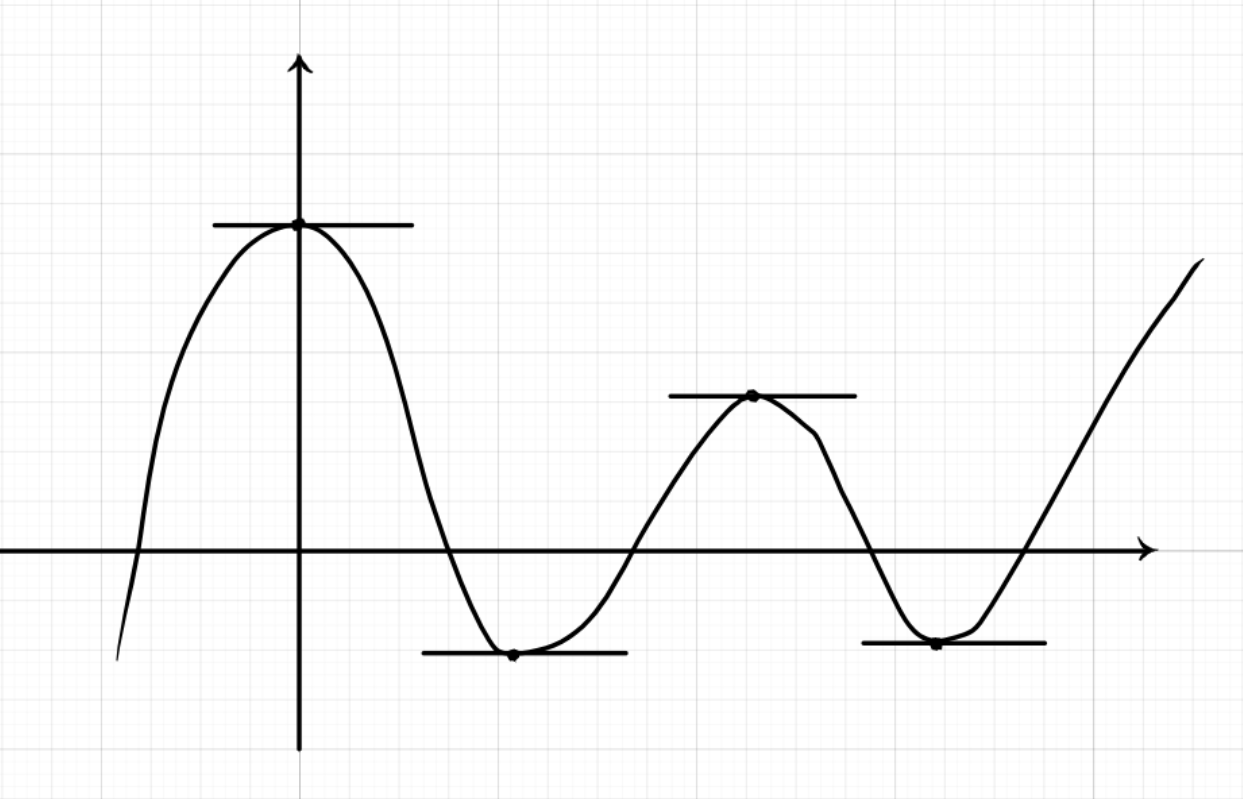
\includegraphics[scale=0.5]{images/img21.png}$$
В точке экстремума касательная к $f$  горизонтальна.\\\\
\textbf{Замечание. Физический смысл.}
При движении по прямой в момент возврата (экстремум!) скорость равна нулю $v = s'(t)$. \\\\
\textbf{Замечаниe.} Если экстремальная точка является граничной, то она может и не быть стационарной точкой, точнее, если $x_0$ --- граничная точка и $f(x_0) = \max f \nRightarrow f'(x_0) = 0.$ 
$$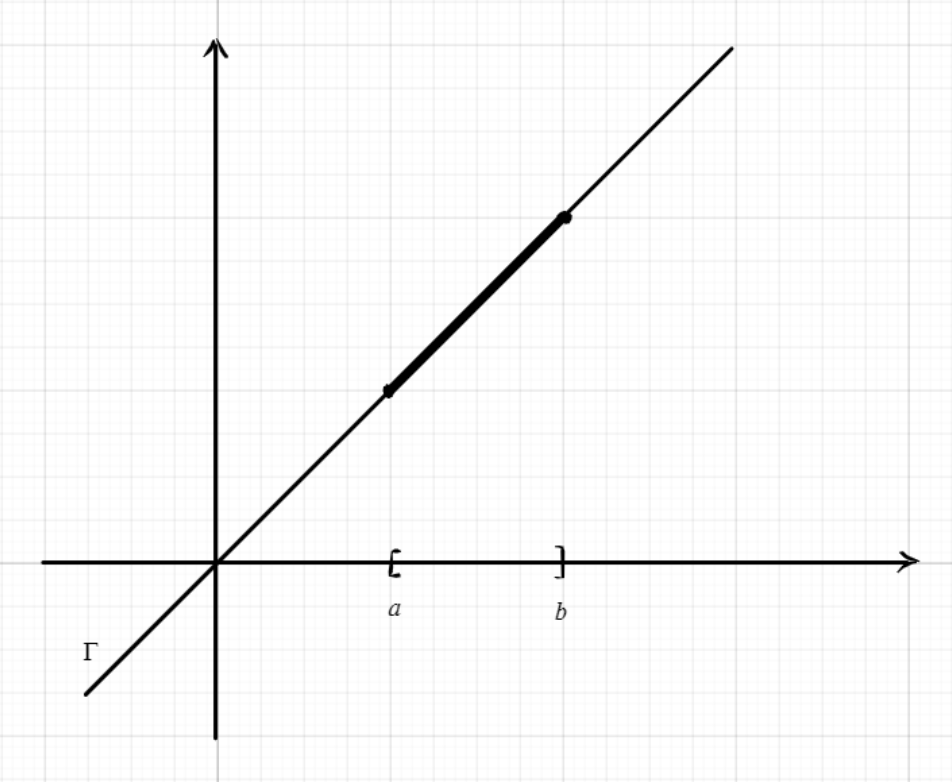
\includegraphics[scale=0.5]{images/img22.png}$$  $f'(a) \neq 0, f'(b) \neq 0.$ \\\\
\textbf{Замечание.} Теорема Ферма даёт только лишь достаточное условие стационарной точки. Обратное, вообще говоря, неверно. Пример: $y = x^3, y'(0) = 0$, однако $x$ не является точкой экстремума.
\newtheorem*{thr}{Теорема Ролля}\begin{thr}
	Пусть $f \in C([a;b]) \wedge f \in D((a;b))$.
	Если $f(a) = f(b)$, то $\exists x_0 \in (a;b)$ что $f'(x_0) = 0$.
\end{thr}
\begin{Proof}
	Так как $f$ непрерывна на отрезке $[a;b]$, то по теореме вейерштрасса она принимает на отрезке $[a;b]$ свои экстремальные значения, то есть $\exists \underline{x}, \overline{x} \in [a;b]$, что $f(\underline{x}) = min f([a;b]), f(\overline{x}) = max f([a;b])$ возможны также варианты: \begin{enumerate}
		\item $ f(\underline{x}) = f(\overline{x}) \Rightarrow f=$ постоянная на $[a;b] \Rightarrow f'(x) = 0, \forall x \in [a;b]$ и в качестве $x_0$ можно взять любую точку из $[a;b]$.
		\item $2) f(\underline{x}) < f(\overline{x})$  Поскольку $f(a) = f(b)$, то по крайней мере одна из точек $\overline{x},\underline{x}$ внутренняя. Её мы обозначим через $x_0$. Функция $f$ дифференцируема в точке $x_0$ на основании условий теоремы $\Rightarrow$ по теореме Ферма $f'(x_0) = 0$.
	\end{enumerate}
\end{Proof}
\subsubsection{Геометрический смысл теоремы.}
$$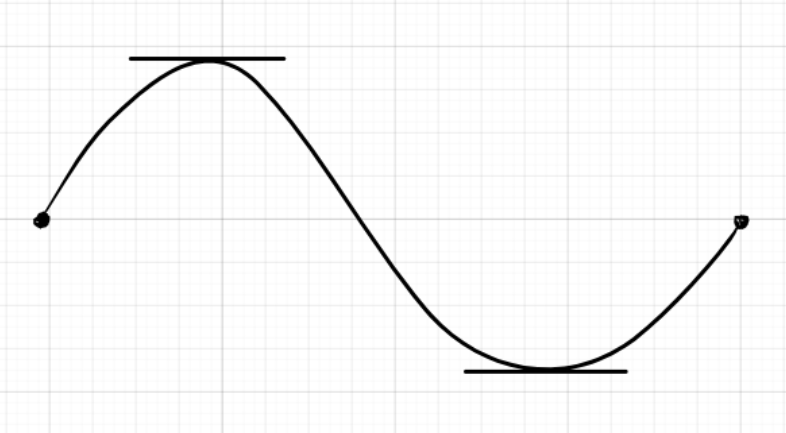
\includegraphics[scale=0.5]{images/img23.png}$$
При выполнении условий теоремы существует точка, в которой касательная горизонтальна.
\subsubsection{Физический смысл теоремы.}
$s(a) = s(b)\Ra$ был момент времени, когда скорость была равна нулю.\\\\
\textbf{Замечание.} Если $f$ непрерывна и дифференцируема, то между нулями функции всегда лежит нуль производной.
\section{Формула конечных приращений.}
\begin{theorem}[Теорема Лагранжа]
	Пусть $f\in \mathcal{C}([a;b])$, $f \in D([a;b])$. Тогда $\exists \xi  \in ]a;b[$ такое, что $f(b) - f(a) = f'(\xi)(b-a)$.
	\end{theorem}
\begin{Proof}
	Введем вспомогательную функцию $$\phi (x) :: =(f(x) - f(a))(b-a)-(f(b)-f(a))(x-a),\ \phi \in \mathcal{C}([a;b]),\ \phi \in D([a;b]),$$
	как линейная комбинация функций, обладающих теми же свойствами.\\\\
	Убеждаемся проверкой, что $\phi (a) = \phi(b) = 0$. По теореме Ролля на $]a;b[$ $\exists \xi : \phi^\prime (\xi) = 0$. Поскольку $\phi^\prime (x) = f^\prime (x)(b-a) - f(b) - f(a)$, то $f^\prime(\xi)(b-a) = f(b) - f(a)$.
	\end{Proof}
\section{Замечания к теореме Лагранжа.}
\begin{enumerate}
	\item \textit{Геометрический смысл теоремы.}\\\\
	Посмотрим внимательно на формулу из теоремы Лагранжа, записиав её в виде
	$$f'(\xi) = \frac{f(b) - f(a)}{b - a}.$$
	Левая часть этой формулы --- это угловой коэффициент к графику функции в точке $(\xi; f(\xi))$.
	$$\tg\alpha = f'(\xi).$$
	Правая часть --- угловой коэффициент хорды, соединяющей точки графика $(a; f(a))$ и $(b, f(b))$.
	Таким образом, угловой коэффициент касательной равен угловому коэффициенту хорды. Это означает, что на графике функции существует точка, в которой касательная параллельна указанной выше хорде.
	$$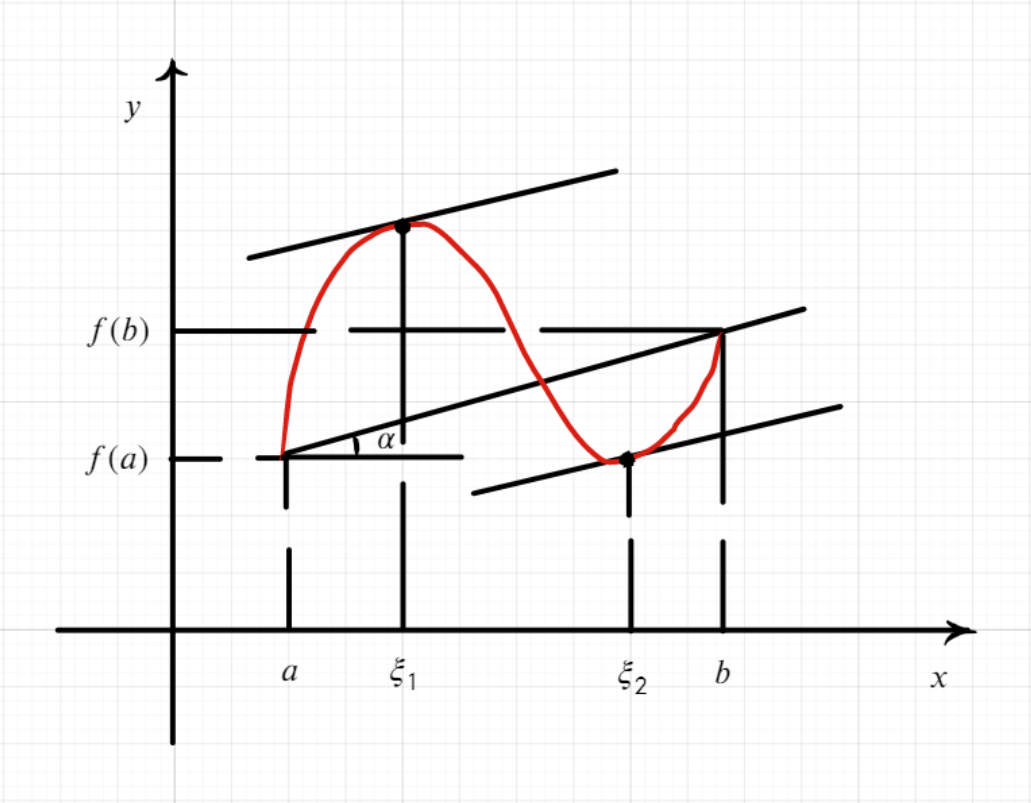
\includegraphics[scale=0.5]{images/img24.png}$$
	\item Умножим формулу на $-1$.\\
	Тогда $f(a) - f(b) = f'(\xi)(a - b)$. Таким образом, в формуле всё равно: $a < b$ или $a > b$.
	Теорема Лагранжа справедлива на отрезке с концами $a$ и $b$.
	\item \textit{Другие формы записи формулы Лагранжа.}\\\\
	Пусть $x$ и $x + h$ принадлежат отрезку $[a;b]$. Если для $f$ выполнены условия теоремы на $[a;b]$, то очевидно, что эти условия выполняются и на отрезке с концами $x$ и $x + h$. Применив теорему Лагранжа на этом отрезке, получаем, что
	$$f(x + h) - f(x) = f'(\xi)h$$
	либо $\Delta x = h$
	$$f(x + \Delta x) - f(x) = f'(\xi)\Delta x$$
	или $$\fbox{$\Delta f = f'(\xi) \Delta x$}$$
	Отсюда и название $"$формула конечных приращений$"$. Она связывает приращение функции на конечном отрезке с производной функции в некоторой точке этого отрезка.
\end{enumerate}
До сих пор мы рассматривали только локальное (бесконечно малое) приращение функции через производную или дифференциал в фиксированной точке.\\\\
Отметим также, что $\xi$ можно представить в виде $\xi = x + \theta \cdot h$, где $\theta$ --- некоторое число.
Тогда
$$f(b) - f(a) = f'(a + \theta (b - a) \cdot (b - a),$$
$$
f(x + h) - f(x) = f'(x + \theta h) \cdot h,$$
$$
f(x + \Delta x) - f(x) = f'(x + \theta \Delta x)\cdot \Delta x.$$
\section{Критерий постоянства дифференцируемой функции.}
\begin{theorem}
	Для того, чтобы дифференцируемая на интервале функция была постоянной на этом интервале, необходимо и достаточно, чтобы $f'=0$ на $]a;b[$.
\end{theorem}
\begin{Proof} 
	\textbf{Необходимость}. $f = C \Rightarrow f' = 0$. \\\\
	\textbf{Достаточность}.
	Дано $f'(x)=0, \forall x \in ]a;b[$. Возьмем $\forall x \in ]a;b[$. Вычислим $f(x_0)$ и покажем, что $f(x) = f(x_0), \forall x \in ]a;b[$.\\\\
	Возьмем $\forall x \neq x_0, x \in ]a; b[$ и применим теорему Лагранжа на отрезке с концами $x$ и $x_0$. Получим $f(x)- f(x_0) = f'(\xi)(x- x_0) = 0 \Rightarrow f(x) = f(x_0)$.
\end{Proof}\\\\
\textbf{Замечание}. Если $f \in C([a;b]) \wedge f \in D(]a;b[)$, то для постоянства $f$ на $[a;b]$ необходимо и достаточно, чтобы 
$f'=0$ на $]a;b[$.\\\\ Доказательство этого утверждения очевидно.
\newtheorem*{thofs}{Теорема о функциях с совпадающими производными}
\begin{thofs}
	Функции $f$ и $g$, обладающие на $]a;b[$ одинаковыми производными, то есть $f'=g', \forall x \in ]a;b[$ отличаются друг от друга на постоянную величину: $f(x) = g(x) + C, \forall x \in ]a;b[$.
\end{thofs}
\begin{Proof}
	$h::=f-g$. $h'= f'-g'=0 \Rightarrow h = C$
	$\Rightarrow f-g=C \Rightarrow f= g+C.$
\end{Proof}\\\\
\textbf{Замечание}. $f, g\in C([a;b]) \wedge f, g \in D(]a;b[), f'=g', \forall x \in ]a;b[$
$ \Rightarrow \exists c, f(x)=g(x)+С, \forall x \in [a;b].$\\\\ Доказательство этого утверждения очевидно.\\
\begin{example}
	$f(x)=\arcsin x, g(x)= -\arccos x$ на $[-1;1]$.
	$$f'(x)=g'(x)=\frac{1}{\sqrt{1-x^2}} \Rightarrow
	\arcsin x + \arccos x = C.$$ $$x = 0 \Rightarrow \frac{\pi}{2} = C \Rightarrow
	\arcsin x + \arccos x = \frac{\pi}{2}=2, \forall x \in [-1;1].$$
\end{example}
\section{Первообразная для функции и дифференциальное выражение.}
Рассмотрим функцию $ f: ]a;b[\rightarrow \Rm $.\\\\
$\bullet$ \textit{Дифференцируемая функция $\mathcal{F}:]a;b[\rightarrow \Rm$ называется \textbf{первообразной} для $f$ на $]a;b[$, если $\mathcal{F}'=f$ для $\forall x \in X$.}\\\\
Если $\mathcal{F}$ --- первооббразная для $f$, то тогда $d\mathcal{F} = \mathcal{F}'(x)dx = f(x)dx$. Поэтому $\mathcal{F}$ называют также \textbf{первообразной и для дифференциального выражения} $f(x)dx$.\\\\
Понятие первообразной можно ввести и на отрезке, если $f$ и $\mathcal{F}$ определены на $[a;b]$, причём $\mathcal{F}$ непрерывна на $[a;b]$, дифференцируема на $]a;b[$.\\
\begin{example}
	$$f=\sin x \rightarrow \mathcal{F}_1 = -\cos x, \mathcal{F}_2 = 2-\cos x$$
	$$f=\frac{1}{1 + x^2} \rightarrow \mathcal{F}_1 = \arctg x, \mathcal{F}_2 = - \mathrm{arcctg}x.$$
\end{example}
\newtheorem*{thoovp}{Теорема об общем виде первообразной}
\begin{thoovp}
	Если $f : X \rightarrow \Rm $, где $X$ --- промежуток, имеет первообразной некоторую функцию $\mathcal{F}$, то $\Phi$ на этом же промежутке будет первообразной для $f$ тогда и только тогда, когда $\Phi = \mathcal{F} + C$, $x \in X$, C --- постоянная. 
\end{thoovp}
\begin{Proof}
	Так как $\mathcal{F}$ первообразная для $f$ на $X$, то $\mathcal{F}' = f$. Тогда $\Phi ' = (\mathcal{F} + C)' = \mathcal{F}' = f$. То есть $\Phi$ также является первообразной.\\\\
	Наоборот. Пусть $\mathcal{F}$ и $\Phi$ две первообразные для $f$ на $X$. Тогда $\mathcal{F}' = f$ и $\Phi ' = f$. Таким образом, у $\mathcal{F}$ и $\Phi$ на промежутке $X$ совпадают производные. А тогда по теореме о функциях с совпадающими производными сами функции отличаются лишь на постоянную, то есть $\mathcal{F} = \Phi + C$.
\end{Proof}\\\\
$\bullet$ \textit{Выражение $\mathcal{F}(x) + C$ называют \textbf{общим видом первообразной}.}